\documentclass{scutthesis} % 不填充空白页。如果需要双面打印版,请注释掉本行并启用下一行
%\documentclass[print-both-sides]{scutthesis} % 使用双面打印版(填充额外空白页以保证每一章开头都在奇数页)
% 开始使用该模板请修改以下文件
%%
% 论文相关信息
% 本文档中前缀"c-"代表中文版字段, 前缀"e-"代表英文版字段
%%

% 标题
% 论文题目应突出重点、简明扼要,能恰当概括论文主要内容,要有较强的科学性和前瞻性、可行性,必要时可增加副标题。

\covertitlefirst{基于卷积神经网络的手写数字及写字人识别}
\covertitlesecond{本科毕业论文(设计)}


\etitlefirst{}
\etitlesecond{}

% 中文标题
\ctitle{基于卷积神经网络的手写数字及写字人识别}
\etitle{}

% 作者详细信息
\author{王小明}
\cauthor{王\ 小\ 明}    % 封面作者
\eauthor{Wang Xiaoming}
\studentid{12350004}
\cschool{计算机学院}

\cmajor{计算机科学与技术}
\emajor{Computer Science and Technology}

% 指导老师
\cmentor{王大明 \ (教授)}
\ementor{Prof. 王大明}

     % 在这里填写论文相关信息
%%
% 摘要信息
% 本文档中前缀"c-"代表中文版字段, 前缀"e-"代表英文版字段
% 摘要内容应概括地反映出本论文的主要内容,主要说明本论文的研究目的、内容、方法、成果和结论。要突出本论文的创造性成果或新见解,不要与引言相 混淆。语言力求精练、准确,以 300—500 字为宜。
% 在摘要的下方另起一行,注明本文的关键词(3—5 个)。关键词是供检索用的主题词条,应采用能覆盖论文主要内容的通用技术词条(参照相应的技术术语 标准)。按词条的外延层次排列(外延大的排在前面)。摘要与关键词应在同一页。
%%

\cabstract{

    炔烃和叠氮化合物的点击化学反应,有着快速、百分百原子利用率、产物高选择性等众多优点,被誉为点击化学中的精华。基于此反应拓展而来的点击聚合反应,迅速在高分子材料领域获得了了广泛关注和应用。
    ……
    我们还尝试了采用不同单体,在最优条件下进行反应,均获得了高分子产物。表明了该反应体系的普适性。

}
% 中文关键词(每个关键词之间用“,”分开,最后一个关键词不打标点符号。)
\ckeywords{多变量系统;预测控制;环境试验设备}

\eabstract{
    % 英文摘要及关键词内容应与中文摘要及关键词内容相同。中英文摘要及其关键词各置一页内。
    Artificial Neuron Network (ANN) simulates human being's brain function and build the network structure. Convolutional Neural Network (CNN) have many advantage, such as ……
    (2) This paper introduces the common pretreatment method of image, such as collecting image, normalization, graying and binarization. And apply these to the handwritten numeral recognition experiment and handwritten numerals writer recognition experiments.

}
% 英文文关键词(每个关键词之间用,分开, 最后一个关键词不打标点符号。)
\ekeywords{Writer recognition;Convolutional Neural Network;Handwritten character recognition}

     % 在这里填写摘要内容注意华工要求关键词用分号分隔
\begin{document}
% 论文前置部分
\frontmatter
\pagenumbering{Roman}
\makeUndergraduateCover    % 生成封面
\makedisclaim
%\makedisclaim[title.png]            % 生成学位论文原创性声明
% 将title.png替换为自己的签名文件,如果不需要签名的话,可以直接使用\makedisclaim命令
\makeabstract       % 生成中英文摘要
\maketableofcontents        % 生成目录
\makelistoffiguretable % 生成图表目录
% 论文主体部分
\mainmatter
% 引言
% 正文
%%
% 引言或背景
% 引言是论文正文的开端,应包括毕业论文选题的背景、目的和意义;对国内外研究现状和相关领域中已有的研究成果的简要评述;介绍本项研究工作研究设想、研究方法或实验设计、理论依据或实验基础;涉及范围和预期结果等。要求言简意赅,注意不要与摘要雷同或成为摘要的注解。
%%

\chapter{绪论}
%定义,过去的研究和现在的研究,意义,与图像分割的不同,going deeper
\label{cha:introduction}
\section{引言}
\label{sec:background}
当今社会,科技的飞速发展为大家提供了快捷与舒适,但与此同时也增添了在信息安全上的危险。在过去的二十几年来,我们通过数字密码来鉴别身份,但是随着科技的发展,不法分子借用高科技犯罪的案例年年增高,密码被盗的情况时常发生。因此,怎样科学准确的辨别每一个人的身份则成为当今社会的重要问题。
\section{研究背景}
\label{sec:related_work}
随着科技的日益发展,传统的密码因为记忆的繁琐以及容易被盗,似乎已经不再能满足这个通信发达的社会的需求。人们急需一种更便捷而且辨识度更高的方式来辨识身份。循着便捷与辨识度高这两个约束条件\overcite{ref1},我们联想到的便是存在于每个人身上的生物特征,所以基于每个人身上不同的生物特征而研究的鉴别技术现在成为了身份辨别技术上的主流。

\section{研究现状}
笔迹获取的方式有两种,所以鉴别方式也分为离线鉴别和在线鉴别\overcite{ref2,ref3}。在线鉴别是采用专用的数字板来实时收集书写信号。由文献\cite{ref4,ref5,ref6,ref7}可知,因为信号是实时采集的,所以能采集的数据不仅包括笔迹序列,而且可以采集到书写时的加速度、压力、速度等丰富有用的动态信息。

\section{论文结构}
本文分为四章。其中第一章简述了笔迹识别的研究背景和意义以及笔迹识别的基础知识等。第二章节从卷积神经网络的发展历史、网络结构、学习规律三方面详细的讲述了卷积网络的基础知识。第三章针对本文中的手写数字及写字人实验具体设计卷积神经网络的网络结构以及训练过程。第五章节是手写数字识别及写字人识别实验的结果与分析。 % 使用include导入章节tex文件
\newclearpage
\chapter{第二章	卷积神经网络的基础知识}
\section{卷积神经网络的网络结构}
卷积神经网络作为深度学习的一个分支,在网络结构上同样含有深度学习的“深度”性。网络拓扑结构是一个多层的神经网络\overcite{ref8},网络的每一层由多个独立的神经元组成的二维平面组成。网络一般分为输入层、卷积层、池化层、全连接层、输出层等。
\subsection{输入层}
因为卷积神经网络可以直接的接受二维的视觉模式\overcite{ref9},所以我们可以直接把简单预处理后的二维图像输入到输入层中。
\subsection{输出}
……
\section{卷积神经网络的学习规律}
……
\subsection{前向传播}
如果用$l$来表示当前的网络层,那么当前网络层的输出如\autoref{eq:fp}所示:
\begin{equation}
    \label{eq:fp}
    {x^l} = f({u^l}),\text{其中}{u^l} = {W^l}{x^{l - 1}} + {b^l}
\end{equation}
其中$f(\cdot)$为网络的输出激活函数。在本文实验中,网络的输出激活函数选用sigmoid函数,因此网络的输出均值一般来说趋于0。
\subsection{反向传播}
……
\subsection{学习特征图的组合}
……
\section{本章小结}
……
\newclearpage
\chapter{\LaTeX 模板配置与使用}
\section{输入输出层的设计}
\section{隐藏层的设计}
\section{本章小结}

\newclearpage
\chapter{第四章	手写数字及写字人识别实验过程及其结果}
\section{手写数字识别实验}
\subsection{样本简介}

本论文的手写数字识别实验当中所用的样本分为两类,一类是训练样本集,另一类是测试样本集。
实验当中的训练样本集采用的是手写数字MNIST数据库。这个数据库当中包含训练集样本60000个样例和测试集样本10000个样例。MNIST数据库当中的数字样本已经全部大小归一化灰度化并且集中到同一个固定大小的图像当中。该数据库包括MST的SD-1和SD-3数据库,当中包含一系列的二级制的手写数字图像。其中SD-1的收集者来源是某高中的在校学生,而SD-3是由人口调查局员工收集的。则我们的训练样本集也就是MNIST当中的训练样本集有30000个样本来自SD-3,而另外30000个样本来自SD-1。这60000个训练样本分别来自约250个采集者。
\subsection{Writer Depend类数字识别实验}
\subsubsection{ABCvsA数字识别实验}
实验内容:以A写字人、B写字人和C写字人,合计3000个数字0到9的数字图像数据为训练样本集。A写字人的1000个数字0到9的数字图像数据为测试样本集。学习率为1,单次训练样本数为10个,共训练40次。若识别所得数字与给定的标签匹配,则视为正确;不匹配则视为错误。
\begin{table}[htbp]
    \centering
    \caption{ABCvsA数字识别实验结果}
    \label{tab:1}
    \begin{tabular}{@{}cccc@{}}
        \toprule
        训练样本 & ABC & 样本个数    & 3000    \\ \midrule
        测试样本 & A   & 样本个数    & 1000    \\
        训练次数 & —   & 单次训练样本数 & 10      \\
        学习率  & 1   & 正确率     & 99.50\% \\ \bottomrule
    \end{tabular}
\end{table}

\subsubsection{ABCvsABC数字识别实验}
实验内容:以A写字人、B写字人和C写字人,合计3000个数字0到9的数字图像数据为总样本集。在总样本集当中随机抽取2400个为训练样本集,余下的600个为测试样本集。学习率为1,单次训练样本数为10个,共训练40次。若识别所得数字与给定的标签匹配,则视为正确;不匹配则视为错误。
\begin{table}[htbp]
    \centering
    \caption{ABCvsABC数字识别实验结果}
    \label{tab:2}
    \begin{tabular}{@{}cccc@{}}
        \toprule
        训练样本 & ABC & 样本个数    & 2400    \\ \midrule
        测试样本 & ABC & 样本个数    & 600     \\
        训练次数 & 40  & 单次训练样本数 & 10      \\
        学习率  & 1   & 正确率     & 92.00\% \\ \bottomrule
    \end{tabular}
\end{table}
\subsection{Writer Depend类数字识别实验结果分析}

下面我们选取Writer Depend类数字识别实验当中的两个典型的例子ABCvsA数字识别实验以及MNIST\&ABCvsA数字识别实验的结果做详细分析。我们从ABCvsA数字识别实验中的训练样本集和测试样本集的手写数字图像样本集当中分别随机抽取一幅图像\ref{fig:complex}所示。

\begin{figure}[htbp] % image examples & compare
    \begin{subfigure}{0.5\textwidth}
        \centering
        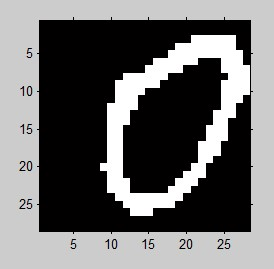
\includegraphics[height=6.54cm]{image/chap04/1.jpg}
        \caption{实验训练集}
        \label{fig:compare1}
    \end{subfigure}
    \begin{subfigure}{0.5\textwidth}
        \centering
        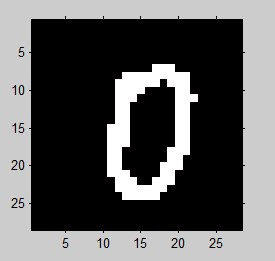
\includegraphics[height=6.54cm]{image/chap04/2.jpg}
        \caption{实验测试集}
        \label{fig:compare2}
    \end{subfigure}
    \caption{ABCvsA数字识别实验集}
    \label{fig:complex}
\end{figure}

下面我们对上述的训练集和测试集进行40次学习率为2,单次训练样本为10的迭代,得到错误率为0.50\%,而其中每次训练时的误差值组成的历史误差值画图分析如下:
……
\subsection{Writer Independ类数字识别实验}
实验内容:以MNIST数据库为训练样本集,共计60000个训练样本。以A写字人合计1000个数字0到9的数字图像数据为测试样本集写字人识别实验
……
\subsection{样本简介}
……
\subsection{两位写字人识别实验}
\subsubsection{单个数字的写字人识别实验}
实验内容:以A写字人,合计800个数字5的数字图像数据加上B写字人,合计800个数字5的数字图像数据,共计1600个样本为总样本集。随机选取其中的1200个样本为训练样本集,其余的400个样本为测试样本集。学习率为2,单次训练样本数为10个,共训练30次。若识别所得写字人与给定的标签匹配,则视为正确;不匹配则视为错误。
\begin{table}[]
    \centering
    \caption{单个数字写字人识别实验结果}
    \label{tab:3}
    \begin{tabular}{@{}cccc@{}}
        \toprule
        训练样本 & A5\&B5 & 样本个数    & 1200    \\ \midrule
        测试样本 & A5\&B5 & 样本个数    & 400     \\
        训练次数 & 30     & 单次训练样本数 & 10      \\
        学习率  & 2      & 正确率     & 99.75\% \\ \bottomrule
    \end{tabular}
\end{table}
\subsubsection{单个数字的写字人识别实验结果分析}

……
\section{本章小结}

……。

\newclearpage
% 论文后置部分
\backmatter
\renewcommand{\chaptermark}[1]{\markboth{\songti #1}{}}
\chapter{结论}
\label{cha:experiment}
\section{论文工作总结}
……
\section{工作展望}
……
 % 制作结论章节
\newclearpage
% 参考文献
\makereferences % 制作参考文献
% 致谢
%%
% 致谢
% 谢辞应以简短的文字对课题研究与论文撰写过程中曾直接给予帮助的人员(例如指导教师、答疑教师及其他人员)表示对自己的谢意,这不仅是一种礼貌,也是对他人劳动的尊重,是治学者应当遵循的学术规范。内容限一页。
% modifier: 黄俊杰
% update date: 2017-04-15
%%

\chapter{致谢}

四年时间转眼即逝,青涩而美好的本科生活快告一段落了。回首这段时间,我不仅学习到了很多知识和技能,而且提高了分析和解决问题的能力与养成了一定的科学素养。虽然走过了一些弯路,但更加坚定我后来选择学术研究的道路,实在是获益良多。这一切与老师的教诲和同学们的帮助是分不开的,在此对他们表达诚挚的谢意。

首先要感谢的是我的指导老师王大明教授。我作为一名本科生,缺少学术研究经验,不能很好地弄清所研究问题的重点、难点和热点,也很难分析自己的工作所能够达到的层次。王老师对整个研究领域有很好的理解,以其渊博的知识和敏锐的洞察力给了我非常有帮助的方向性指导。他严谨的治学态度与辛勤的工作方式也是我学习的榜样,在此向王老师致以崇高的敬意和衷心的感谢。

最后我要感谢我的家人,正是他们的无私的奉献和支持,我才有了不断拼搏的信心和勇气,才能取得现在的成果。

\vskip 108pt
\begin{flushright}
    王小明\makebox[1cm]{} \\
    \today
\end{flushright}

 % 制作致谢
\newclearpage
% 附录部分
% 附录
{
    \appendix
    \renewcommand{\chaptermark}[1]{\markboth{\songti  附录\thechapter\ ~#1}{}}
    \chapter{补充更多细节}

\section{补充图}

\subsection{补充图}

这是附录内容,应该用宋体小四号字体。
\begin{figure}[htbp]
        \centering
        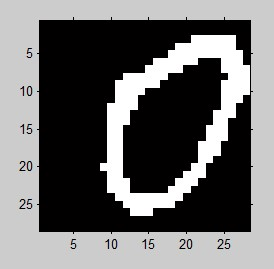
\includegraphics[height=6.54cm]{image/chap04/1.jpg}
        \caption{实验训练集}
\end{figure}
\begin{figure}
        \centering
        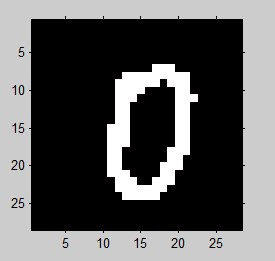
\includegraphics[height=6.54cm]{image/chap04/2.jpg}
        \caption{实验测试集}
\end{figure}

\endinput
 % 导入附录
    \newclearpage
}
\end{document}